\ifdefined\XeTeXversion
  % IEEEtran selects ptm before loading the user preamble. Map its Unicode
  % NFSS families explicitly so XeTeX retains serifs, italics and bold.
  \newcommand{\UXfont}[5]{\DeclareFontShape{TU}{#1}{#2}{#3}{<->"[#4]:mapping=tex-text"}{}}
  \newcommand{\UXfamily}[5]{%
    \DeclareFontFamily{TU}{#1}{}%
    \UXfont{#1}{m}{n}{#2}{}\UXfont{#1}{m}{it}{#3}{}%
    \UXfont{#1}{b}{n}{#4}{}\UXfont{#1}{bx}{n}{#4}{}%
    \UXfont{#1}{b}{it}{#5}{}\UXfont{#1}{bx}{it}{#5}{}%
    \DeclareFontShape{TU}{#1}{m}{sl}{<->ssub*#1/m/it}{}%
    \DeclareFontShape{TU}{#1}{m}{sc}{<->ssub*#1/m/n}{}}
  \IfFileExists{times.ttf}{%
    \UXfamily{ptm}{times.ttf}{timesi.ttf}{timesbd.ttf}{timesbi.ttf}
    \UXfamily{phv}{arial.ttf}{ariali.ttf}{arialbd.ttf}{arialbi.ttf}
    \UXfamily{pcr}{cour.ttf}{couri.ttf}{courbd.ttf}{courbi.ttf}
  }{%
    \UXfamily{ptm}{texgyretermes-regular.otf}{texgyretermes-italic.otf}{texgyretermes-bold.otf}{texgyretermes-bolditalic.otf}
    \UXfamily{phv}{texgyreheros-regular.otf}{texgyreheros-italic.otf}{texgyreheros-bold.otf}{texgyreheros-bolditalic.otf}
    \UXfamily{pcr}{texgyrecursor-regular.otf}{texgyrecursor-italic.otf}{texgyrecursor-bold.otf}{texgyrecursor-bolditalic.otf}
  }
\fi
\documentclass[conference]{IEEEtran}
\usepackage[brazilian]{babel}
\usepackage{array,tabularx,amsmath,graphicx}
\newcommand{\institution}{CEFET-MG, Campus Divinópolis, Engenharia de Computação}
\newcommand{\groupauthors}{\IEEEauthorblockN{Élcio Costa Amorim Neto, Guilherme Alvarenga de Azevedo e Joaquim Cézar Santana da Cruz}\IEEEauthorblockA{\institution}}
\addto\captionsbrazilian{\renewcommand{\abstractname}{Resumo}\renewcommand{\refname}{Referências}}
\renewcommand{\IEEEkeywordsname}{Palavras-chave}
\newcommand{\UXev}[1]{\textsf{\detokenize{#1}}}
\newcommand{\UXrow}[2]{\noindent\begin{tabularx}{\columnwidth}{@{}>{\raggedright\arraybackslash}p{.30\columnwidth}>{\raggedright\arraybackslash}X@{}}\textbf{#1} & #2\end{tabularx}\par}
\newenvironment{uxtable}[2]{\par\smallskip\begingroup\footnotesize\setlength{\parskip}{1pt}\setlength{\tabcolsep}{3pt}\hrule\nobreak\UXrow{#1}{\textbf{#2}}\nobreak\hrule\nobreak}{\nobreak\hrule\endgroup\par\smallskip}

\AtBeginDocument{\raggedbottom}


\title{Caderno de especificação de design do UX-Agent\\Cardápio móvel, canal de observação e conferência do pedido}
\author{\groupauthors}
\begin{document}\maketitle
\begin{abstract}Este caderno reúne os modelos e decisões usados para construir as duas versões do cardápio. As tarefas C1 e C2 vinculam o protocolo ao piloto de instrumentação. As árvores de V1 e V2 documentam o protocolo reservado para uma avaliação futura. A leitura conjunta das falas, dos signos e dos eventos permite verificar o que cada receptor pode perceber, quais ações estão disponíveis e como o pesquisador reconstrói o resultado.\end{abstract}
\section{Do modelo ao design}
A reformulação reflexiva do problema \cite{schon} orientou a passagem das metas às condições verificáveis. O problema proposto na Fase I \cite{fase1} ganhou precisão com a curadoria \cite{pesquisa}, a modelagem das tarefas e telas \cite[apêndices B e C]{modelagem} e a especificação do protocolo \cite[pp.~1--8]{hts}. T1--T4 passaram a C1, C2, V1 e V2, e as variantes V2/V6 passaram a P2/P6. V1/V2 foram congeladas em 26/10/2026. Usamos E para Evidência, PD para Princípio de Design e HO para Hipótese Operacional.
\begin{uxtable}{Dimensão}{Formulação atual e reformulação}
\UXrow{T, tecnologia}{Cardápio web fictício, 30 itens e duas versões. Instrumentar a aplicação passou a ser condição para medir o estado fora do agente.}
\UXrow{U, pessoas}{Adultos de 18 a 59 anos com baixa visão moderada a grave, campo preservado e leitura com ampliador. A geometria aproxima a vista ampliada.}
\UXrow{C, contexto}{Almoço no escritório e jantar em casa. A sessão individual preserva o combinado e o orçamento. Interrupções, luz ambiente e pagamento ficam fora do estudo.}
\UXrow{I, investigação}{Deslocamento, revisita, associação e conferência substituíram tempo e carga percebida, que exigiriam dados específicos ou relato humano.}
\UXrow{G, lacuna}{A literatura consultada carece de comparação humana nas mesmas tarefas em smartphone. A primeira função do protótipo passou a ser testar a integridade do instrumento.}
\end{uxtable}
\textit{Elenco.} Lívia é uma personagem fictícia de 34 anos, assistente administrativa. Sua baixa visão congênita corresponde, na ficha, a acuidade 0,1 (20/200) no melhor olho e campo preservado. Usa fonte grande e ampliador Android de tela cheia, lê fluentemente quando a palavra cabe na vista e compara o que consegue reunir. A irmã inicia um pedido e o companheiro compartilha restrições no jantar. O atendente receberia o pedido no contexto real. O moderador futuro observa e o pesquisador audita. O comparador humano proposto corresponde a adultos sem baixa visão pareados por idade, escolaridade e uso diário de smartphone. O recorte exclui pessoas cegas, usuárias de leitor de tela, com perda predominante de campo visual, deficiência motora associada ou idade a partir de 60 anos.
A modelagem herdada situa o recorte nos códigos CID-11 9D90.2 e 9D90.3 e documenta a referência ao Decreto brasileiro nº 5.296/2004 \cite[pp.~3, 10--11]{modelagem}. Essa descrição delimita o público da pesquisa. Os parâmetros do controlador são escolhas operacionais.
\par E: há alternância entre alvo e contexto \cite[p.~9]{billah}, diferentes níveis de ampliação e estratégias de varredura \cite[pp.~12, 20, 25]{islam}. HO: a transferência dessas observações a um cardápio, os limiares de legibilidade e a capacidade da memória simulada. P sorteia $z$ de 3 a 5 e usa varredura linear. P2 e P6 sorteiam $z$ de 1,5 a 2,5 e de 5,5 a 7, respectivamente. Nas variantes, a probabilidade de varredura linear é 9/11. C inicia em $z=1$, com varredura livre e sem deslize. Os quatro perfis compartilham $k\in\{3,4,5\}$, $n=5$ e $q=0{,}5$. G é o controle genérico de página inteira. R executa o método especialista.
\par\textit{Especificação de usabilidade.} Eficácia significa entregar a composição desejada. Segurança implica reconhecer e reparar um engano antes de confirmar (PD). Em C1/C2, a aceitação técnica de R exige $S=1$, ausência de E1--E6 e $R_A=1$. Eficiência é expressa em ações por execução e deslocamentos por item. Utilidade exige um caminho para cada uma das quatro intenções. Aprendizagem requer treino em outro cardápio e ajuda procedimental. Facilidade de lembrar requer reconsulta a itens, pedido e instrução. Autonomia e confiança orientam a edição e o suporte. Sua avaliação exige pessoas. Para o estudo futuro, as tolerâncias para o erro da diferença P--C são 1,5 ação/item em $D$, 0,15 em $Re_{E5}$ e 0,20 em $S$ \cite[p.~7]{hts}. A decisão considera o sinal da diferença e a posição do intervalo de 90\%.
\par\textit{Restrições.} As versões conservam itens, preços, opções, objetivos, condições iniciais e ajuda. O comparador futuro requer informação disponível, ações essenciais e prevenção equivalentes. A composição visual é livre somente enquanto preservar os signos relevantes. A interface de uma amostra humana independente é desconhecida. Calibração usa C1/C2. O treino usa cinco lanches e o único exemplo funcional emprega pão de queijo.
\section{Metamensagem e dois receptores}
\textit{Metamensagem do designer.} Entendo que você quer pedir sua própria refeição e conferir a de quem vai comer com você. Você costuma ampliar o que lê e pode perder de vista a relação entre um prato e seu preço. Por isso, reuni nome, opções e preço junto de cada escolha. Você pode voltar a eles, conferir o que já incluiu e corrigir o pedido antes de registrá-lo. Quando quiser entender uma opção, há uma explicação no ponto em que a dúvida surgiu. A interface funciona como preposto do designer \cite{desouza}. Essa perspectiva comunicativa admite manipulação direta \cite[p.~230]{barbosa}.
\begin{uxtable}{Jakobson}{Persona / agente e diferença declarada}
\UXrow{Emissor}{O designer se manifesta em preços, escolhas e respostas. O mesmo preposto produz a próxima observação. PD: autoria comum.}
\UXrow{Receptor}{Lívia interpreta com sua experiência. O modelo escolhe uma ação do recorte recebido. HO: representação funcional.}
\UXrow{Contexto}{A pessoa reconhece a ocasião e lê o combinado. O agente recebe a mesma instrução. HO: ruído, pressa e companhia ficam fora da sessão.}
\UXrow{Código}{Português, moeda, etiquetas, posição e controles. O agente lê fragmentos e coordenadas. HO: perde parte das pistas de tipografia e cor.}
\UXrow{Canal}{Lívia acompanha uma região ampliada e desloca a vista. O executor transmite interseções legíveis e memória limitada. HO: aproximação geométrica.}
\UXrow{Mensagem}{Escolher, conferir, corrigir e registrar uma refeição. O registro comunica o fim a ambos. PD: o verificador compara a composição final com o objetivo.}
\end{uxtable}
\textit{Modelo conceitual.} O cardápio apresenta o que a cozinha oferece. O pedido em andamento funciona como uma comanda editável. Repetir um pedido anterior acrescenta suas linhas à comanda atual. Confirmar encerra a edição. A metáfora termina no registro: estoque, atendimento de cozinha e pagamento ficam fora do sistema. C1 explora e navega pelas massas. C2 manipula quantidades após comparar linhas. V1 explora combinações e manipula a composição. V2 instrui a cópia e manipula uma linha. Categorias, linhas e quantidades são conceitos. Lista, abas, rodapé e controles são expressões físicas \cite[p.~199]{benyon}.
\section{Objetivos e cenários de interação}
Os cenários descrevem intenções, consequências e alternativas antes da escolha das expressões físicas \cite{rosson}.
\begin{uxtable}{Objetivo final}{Papel, entidade e objetivos instrumentais}
\UXrow{F1 Almoçar dentro do combinado}{Lívia / refeição individual. Direto: obter a porção de menor preço. Indireto: conhecer preços de porções comparáveis.}
\UXrow{F2 Receber a refeição combinada}{Lívia e irmã / pedido iniciado. Direto: adequar a composição. Indireto: conhecer divergências.}
\UXrow{F3 Jantar a dois dentro do orçamento}{Lívia e companheiro / jantar. Direto: conciliar itens e quantidades. Indireto: conhecer ingredientes e custo.}
\UXrow{F4 Compartilhar o jantar habitual}{Lívia e irmão / pedido anterior. Direto: adequar a porção preservando o restante. Indireto: reconhecer alimentos anteriores.}
\end{uxtable}
\textit{S1, almoço.} Com pouco tempo, Lívia procura massas e compara o preço de três lasanhas individuais. O restaurante apresenta o preço de cada porção consultada. Ela reúne as informações, escolhe a de menor valor e confere o que será preparado. O restaurante registra a refeição.
\par\textit{S2, pedido da irmã, alternativa A.} Lívia pede que o restaurante apresente o que já foi encomendado. Percorre os alimentos um a um, identifica a diferença na sobremesa e solicita a correção. O restaurante apresenta a nova quantidade e o custo. Ela volta a conferir e autoriza o preparo.
\par\textit{S2, alternativa B.} Enquanto considera as escolhas, Lívia pode acompanhar a composição e o valor do que já foi encomendado. Quando a informação escapa da sua vista, ela a procura novamente. Compara o que encontra com o combinado, corrige a quantidade e verifica o resultado antes de autorizar o preparo. O restaurante registra a composição final.
\par\textit{S3, jantar.} Lívia e o companheiro querem dois pratos principais vegetarianos, duas bebidas sem açúcar e uma sobremesa. O restaurante informa ingredientes e preços à medida que ela os solicita. Ela confronta a refeição com o limite de R\$\,110,00, substitui escolhas se necessário e autoriza o preparo.
\par\textit{S4, repetição.} Lívia quer servir ao irmão o jantar da semana anterior, com uma porção maior de macarrão. O restaurante recupera a composição passada. Ela pede para repeti-la, ajusta a porção, compara a refeição atual com a anterior e dispensa o que estava a mais. O restaurante registra o jantar.
\begin{uxtable}{Problema}{Interação $\rightarrow$ tarefa $\rightarrow$ objetivo final}
\UXrow{S1, intervalo curto}{Comparar porções no almoço $\rightarrow$ C1 $\rightarrow$ F1.}
\UXrow{S2, pedido iniciado}{Conferir em separado ou acompanhar a composição $\rightarrow$ C2 $\rightarrow$ F2.}
\UXrow{S3, restrições}{Conciliar composição e custo $\rightarrow$ V1 $\rightarrow$ F3.}
\UXrow{S4, repetir jantar}{Reconstruir e ajustar $\rightarrow$ V2 $\rightarrow$ F4.}
\end{uxtable}
A cena crítica revelou duas perguntas. O resumo continua perceptível quando a pessoa amplia outra região? A área dedicada a ele prolonga a busca? O protocolo registra exposição e deslocamentos. Ambas são HO e precedem o exame de V1/V2.
\section{Signos e fronteira de observação}
A linha de pedido transforma um alimento do domínio em uma combinação editável de item, opção e quantidade. Um número pode significar unidades da linha, total de unidades ou dinheiro, conforme rótulo e posição. Agrupamento e moeda fazem parte da expressão. O esquema completo no apêndice distingue conteúdo, expressão, origem, tipo, projeção e evento. Um preço parcialmente visível permanece um trecho. A coordenada da quantidade não transporta o nome do item quando este está fora da vista. A memória conserva fragmentos efetivamente vistos. Ícones, pesos e cores têm equivalência parcial (HO). Identificadores internos ficam no registro do pesquisador. G constitui controle de página inteira, distinguível das configurações restritas.
\section{Modelos temporais e procedimentais}
As árvores no apêndice refinam a HTA \cite[pp.~3, 5, 8--9]{hts} por responsabilidade e ordem \cite[cap.~4, pp.~39--66]{paterno}. A leitura mental não produz evento. A exposição do signo registra uma oportunidade de leitura. A operação de conferir em C2 começa pelo acesso à revisão descrito na HTA. A narrativa também descreve a revisão deixada aberta. Fixamos o início mensurado com o pedido carregado e um acesso à revisão, para conservar as três ações de referência (HO). V1 conserva as três categorias permutáveis e a repetição em caso de divergência. V2 conserva a espera pelo carregamento, a reconsulta opcional e a remoção do residual.
\par\textit{CMN-GOMS de C1.} Obter a lasanha individual de menor preço requer localizar massas, comparar três pares nome--preço, escolher, compor e confirmar. Os operadores observáveis são deslocar, abrir item, escolher porção, adicionar, abrir revisão, voltar e confirmar. Comparar é interno. Método direto: chegar às massas pela lista (A) ou categoria (B), ler três preços, abrir a escolhida, selecionar a porção individual, adicionar, rever e confirmar. Método por detalhes: para cada preço ilegível, abrir o item, ler e voltar antes de decidir. A regra de seleção é a legibilidade do preço no contexto do nome. Três consultas acrescentam três aberturas e três retornos. A sequência de telas permite identificar o método. No direto, há cinco toques em A ou seis em B, além dos deslocamentos determinados pela geometria. Em C2, corrigir uma unidade da linha exige menos operações que remover e recompor a linha; ambos constituem métodos admissíveis \cite[cap.~5, pp.~139--192]{card83}.
\par\textit{Comparação KLM na cena crítica.} Adota-se uma única tabela \cite[p.~399, Tabela~I]{card80}: apontar $P=1{,}10$~s, acionar $K=0{,}20$~s, preparar $M=1{,}35$~s. A aproximação de um toque por $PK$ é HO. Inserimos $M$ antes de cada escolha independente e nenhum $M$ entre apontar e acionar o mesmo alvo. Consideram-se alvos localizados, sem deslocamento, resposta sem espera e especialista sem erro \cite[pp.~448--456]{preece}. Para consultar a composição durante a escolha e retomar a seleção, A exige abrir e voltar, $MPK\,MPK=5{,}30$~s. Em B, se o resumo necessário estiver na vista, a consulta não exige acionamento ($0$~s de operadores motores ou de preparação para acioná-los). A duração da leitura, exigida nas duas alternativas, é desconhecida. Se o resumo sair da vista, a estimativa perde sua premissa. Na correção integral de C2, restam três escolhas em ambas, $3(MPK)=7{,}95$~s sem deslocamento. A referência observável é $N_{\rm ref}(z)$, contagem de ações do especialista na mesma geometria. A latência do modelo e a duração de uma pessoa com baixa visão não se deduzem dessa tabela. O método especialista também orienta a redação de ajuda procedimental e permite identificar procedimentos discrepantes para operações equivalentes.
\section{Conversa, recuperação e comunicabilidade}
A MoLIC representa o papel de quem faz o pedido \cite{molic}. O executor interpreta transições derivadas desse diálogo. A observação expõe respostas do preposto e ações correntes perceptíveis. O apêndice liga cenas, guardas, processos e recuperações.
\begin{figure}[ht]
\centering
\setlength{\unitlength}{1pt}
\begin{picture}(238,112)
\put(0,87){\framebox(50,18){S0 · Início}}
\put(94,87){\framebox(58,18){S1 · Cardápio}}
\put(188,87){\framebox(48,18){S2 · Item}}
\put(50,98){\vector(1,0){44}}\put(59,101){\scriptsize abrir}
\put(94,91){\vector(-1,0){44}}\put(57,80){\scriptsize início}
\put(152,98){\vector(1,0){36}}\put(154,101){\scriptsize escolher}
\put(188,91){\vector(-1,0){36}}\put(157,80){\scriptsize incluir}
\put(94,40){\framebox(58,18){S3 · Revisão}}
\put(188,40){\framebox(48,18){S4 · Fim}}
\put(123,87){\vector(0,-1){29}}\put(127,69){\scriptsize rever}
\put(113,58){\vector(0,1){29}}\put(64,68){\scriptsize continuar}
\put(152,48){\vector(1,0){36}}\put(151,53){\scriptsize confirmar}
\put(212,87){\line(0,-1){24}}\put(212,63){\line(-1,0){73}}\put(139,63){\vector(0,-1){5}}\put(172,66){\scriptsize salvar}
\put(25,87){\line(0,-1){39}}\put(25,48){\vector(1,0){69}}\put(30,51){\scriptsize repetir ou rever}
\put(0,4){\framebox(101,18){Origem · S0 a S4}}
\put(158,4){\framebox(78,18){S5 · Ajuda}}
\put(101,17){\vector(1,0){57}}\put(110,21){\scriptsize consultar}
\put(158,9){\vector(-1,0){57}}\put(116,0){\scriptsize fechar}
\end{picture}
\caption{Transições principais da implementação. Editar uma linha em S3 reabre S2. Voltar preserva a origem da revisão ou da edição. Confirmar exige comanda não vazia. Uma fala inválida mantém a cena; o suporte restaura a origem.}
\label{fig:estados}
\end{figure}

\begin{uxtable}{Elemento}{Leitura da pessoa / agente / registro}
\UXrow{Cena}{A pessoa reconhece o assunto pelos signos. O agente recebe o recorte. A transição registra a tela anterior e a nova.}
\UXrow{Fala u:}{A pessoa solicita uma operação. O agente escolhe um gesto permitido para um alvo exposto. Registra-se a ação executada.}
\UXrow{Fala d:}{Após alterar uma linha, a pessoa vê sua quantidade. O agente recebe o fragmento exposto. Registram-se mutação e exposição.}
\UXrow{Processo}{A comanda é copiada, recalculada ou registrada. Pessoa e agente recebem o efeito expresso. O verificador lê a composição integral.}
\UXrow{Recuperação}{A pessoa pode voltar aos detalhes ou recompor a linha. O agente vê as mesmas possibilidades. Correções geram alteração, remoção ou adição.}
\UXrow{Acesso ubíquo}{Ajuda suspende a conversa. Fechar devolve à origem. O agente recebe o conteúdo após a abertura. O registro identifica origem, tópico e camada.}
\end{uxtable}
\textit{Matriz de rupturas (PD).} PP antecipa um problema pela expressão, PA restringe uma operação, AL alerta, RA permite corrigir e CE captura uma tentativa inválida. As operações seguem a numeração da HTA \cite[pp.~5, 8--9]{hts}.
\begin{uxtable}{Operação e risco}{Signo, intervenção, evento e métrica}
\UXrow{C1\,1; C2\,2.1; V1\,1--3; V2\,4.1: deslize ou omissão}{Nome e preço agrupados (PP); reconsultar ou voltar (RA). Deslocamento e exposição informam $D,O$. Deslize seguido de retorno informa E4 e $A$.}
\UXrow{C1\,2--3.1; V1\,1--3; V2\,3.1 e 5: seleção ou associação}{Nome junto de preço, etiqueta e controles (PP); rever, remover ou recompor (RA). Adição, alteração e remoção alimentam E1/E2, $V$.}
\UXrow{C1\,3.2--3.3; C2\,3; V1\,1.5--1.7, 2.5--2.6; V2\,3.2--3.3: opção ou quantidade}{Opção exigida e número expostos (PP); a inclusão exige opção (PA); escolher e editar (RA). Seleção e mutação delimitam E3.}
\UXrow{C1\,4; C2\,2.2--4; V2\,4--6: discrepância}{Linhas e total antecipam a consequência (PP); alterar quantidade, reconsultar ou remover (RA). Confirmação e composição final determinam E5; exposição informa $O$.}
\UXrow{V1\,4--5: regra ou orçamento}{Etiquetas e total (PP); substituir antes de confirmar (RA). O orçamento é avaliado externamente. Confirmação e regra determinam E6.}
\UXrow{Tentativa incompatível}{A guarda captura a proposta fora do conjunto permitido (CE); o pedido conserva a composição. A indicação de opção necessária alerta (AL). Contam-se rejeições à parte de $A$.}
\end{uxtable}
Uma PA elimina a oportunidade de efetivar a operação bloqueada. PP e RA preservam erros recuperados. As taxas requerem guardas e denominadores equivalentes no comparador. Alertas sobre uma divergência específica entregariam o critério da tarefa; a interface informa apenas valores e operações.
\par\textit{MAC operacional.} As etiquetas de comunicabilidade \cite{mac} são HO de interpretação do log. \emph{Socorro!} corresponde à abertura de ajuda. \emph{Desisto} corresponde à desistência explícita. \emph{Pra mim está bom} indica confirmação com estado final incorreto. \emph{Epa!} indica deslize seguido em até duas ações executadas de retorno ou correção aplicável. \emph{Cadê?} identifica $n$ ações seguidas sem novo signo, tela ou alteração do pedido, uma ocorrência por sequência. \emph{O que é isso?} indica a abertura da primeira camada de ajuda para um tópico. Duas assinaturas podem coincidir. A atribuição de intenção exigiria investigação com pessoas.
\section{Ajuda sob demanda}
O conteúdo procede dos conceitos, das tarefas e da conversa \cite[pp.~39--55]{silveira}. S5 preserva a origem, oferece dica local, explicação contextual e guia de uso, e termina por decisão da pessoa. A aplicação compartilha uma fonte textual entre a interface humana e a projeção filtrada.
\begin{uxtable}{Dúvida e pergunta}{Modelo e conteúdo}
\UXrow{Informativa: o que oferece?}{Domínio, S1: cada item tem nome, descrição e preço.}
\UXrow{Descritiva: o que é tamanho?}{Signos, S2: tamanho é a porção da massa, distinto da quantidade.}
\UXrow{Procedimental: como editar?}{GOMS, S2/S3: alterar a linha, escolher a opção e salvar.}
\UXrow{De escolha: alterar ou remover?}{MoLIC, S3: alterar edita as opções; remover retira a linha.}
\UXrow{Sugestiva: o que conferir?}{Cenário, S3: conferir nomes, opções e quantidades.}
\UXrow{Investigativa: onde vejo o efeito?}{Processo, S3: a quantidade e o total expressam a mudança.}
\UXrow{Interpretativa: o que é SA?}{Domínio, S1: sem açúcar ou sem açúcar adicionado.}
\UXrow{Navegacional: onde rever?}{MoLIC, S1: a revisão reúne as linhas em andamento.}
\UXrow{Histórica: o que foi repetido?}{Comanda, S0: reconsultar a composição anterior e conferir a cópia.}
\UXrow{De motivação: por que confirmar?}{Metamensagem, S4: confirmar registra e encerra o pedido.}
\end{uxtable}
Os seis requisitos de suporte orientam o projeto \cite[pp.~397--399]{dix}. Disponibilidade: acesso nas cenas da interação. Precisão e completude: cada tópico descreve operações existentes e as camadas cobrem as dez dúvidas. Consistência: títulos e orientações usam o vocabulário das ações. Robustez: ler não altera o pedido e fechar retorna à origem. Flexibilidade: a pessoa escolhe a profundidade. Discrição: o conteúdo aparece após a abertura. M7 age no controlador que representa a pessoa; a interface não possui um assistente adaptativo. Na calibração é permitida a inspeção de entradas, saídas e condição de M7. Na validação futura, conteúdo, regras e parâmetros deverão estar congelados. Para cada camada, contam-se acessos por execução e fração das execuções elegíveis com acesso. A posição do primeiro acesso é o índice da ação dividido pelo número de ações executadas.


\bibliographystyle{IEEEtran}\bibliography{referencias}
\clearpage\appendices
\section{Árvores temporais completas}
\noindent\textbf{Leitura.} A identifica tarefa abstrata, U interna do usuário, I interativa e S do sistema. $\gg$ impõe sequência; $[\,]\gg$ transmite o resultado ao sucessor; $[\,]$ entre tarefas oferece escolha; $|||$ permite intercalação; $|=|$ permite qualquer ordem sem intercalação. Colchetes em torno de uma tarefa indicam opcionalidade e o asterisco indica repetição. Os números recuperam as operações da HTA. Ao ler um cartão de V1, etiquetas $|=|$ preços permite conferir integralmente um ou outro primeiro. O rótulo da apresentação não presume leitura mental.
\par\smallskip Para cada raiz $T$, aplica-se $(T\,|>\,\text{consultar ajuda})\,[>\,(\text{desistir}\,[\,]\,\text{atingir limite}\,[\,]\,\text{falhar})$. A consulta suspende e retoma: solicitar ajuda (I) $\gg$ apresentar dica (S) $\gg$ [escolher camada (I) $\gg$ apresentar conteúdo (S)]* $\gg$ fechar (I) $\gg$ restaurar origem (S). A desativação termina por desistência (I), limite (S) ou falha técnica (S). O suporte fica fora dos métodos especialistas.
\par\smallskip\noindent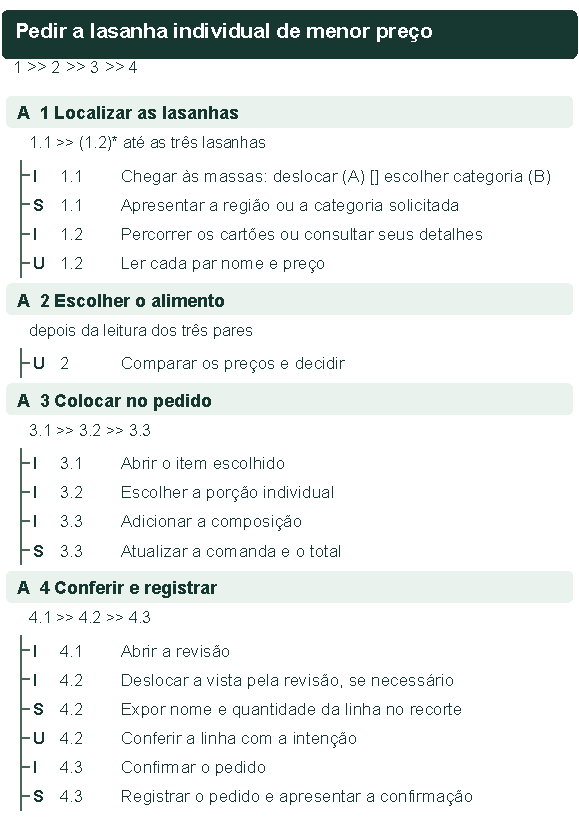
\includegraphics[width=\columnwidth]{../design/figures/CTT-C1.pdf}
\par\smallskip\noindent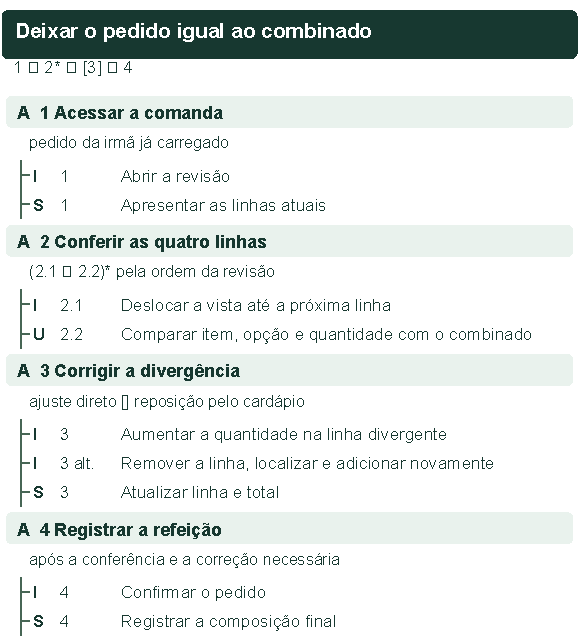
\includegraphics[width=\columnwidth]{../design/figures/CTT-C2.pdf}
\par\smallskip\noindent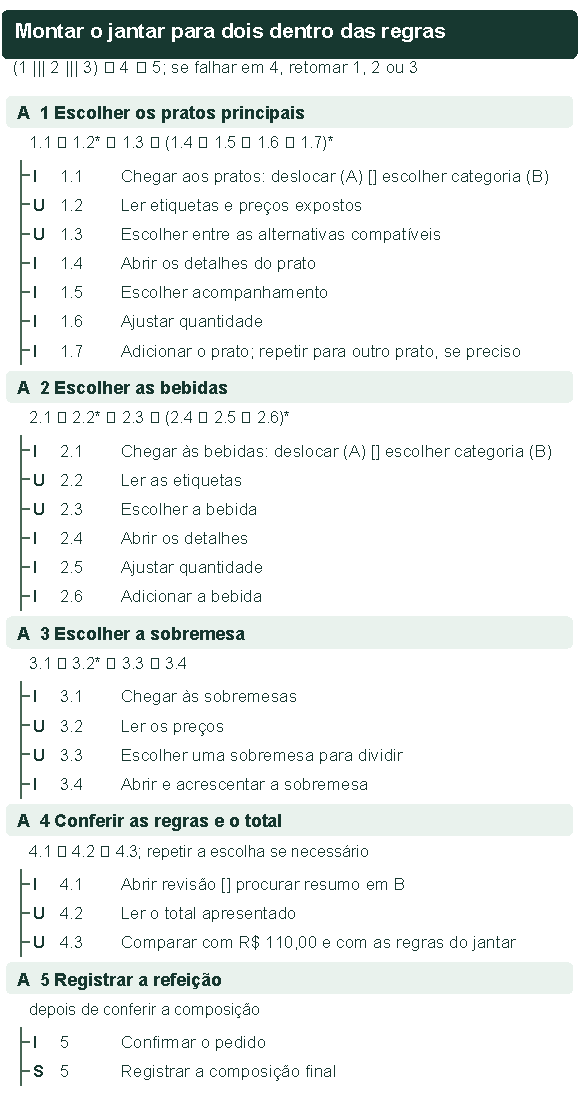
\includegraphics[width=\columnwidth]{../design/figures/CTT-V1.pdf}
\par\smallskip\noindent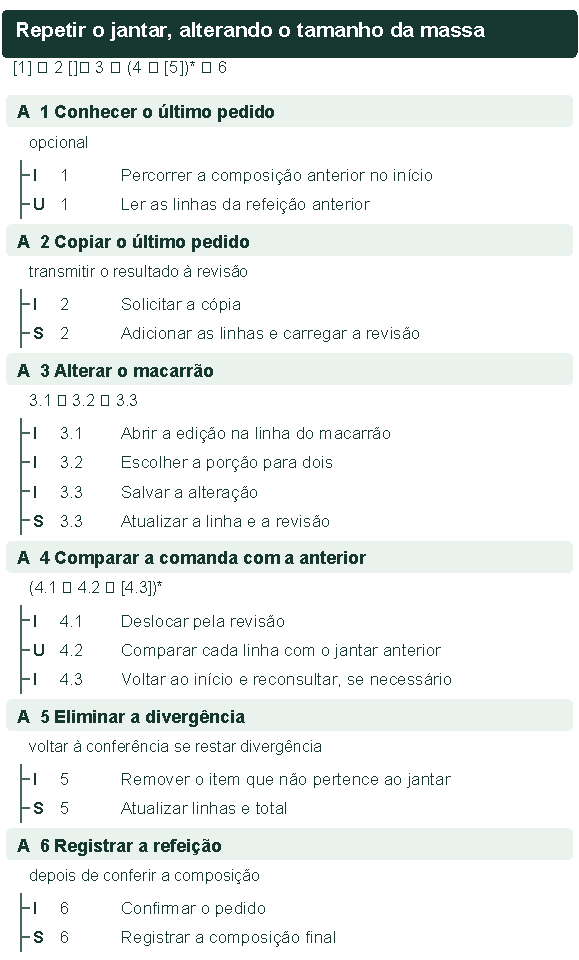
\includegraphics[width=\columnwidth]{../design/figures/CTT-V2.pdf}
\section{Diálogo e esboços do protótipo}
\noindent\textbf{MoLIC.} As cenas delimitam assuntos, P identifica processos e as guardas limitam atos de fala. O subdiálogo S5 preserva a cena de origem. Ajustar a vista conserva o assunto corrente. A desistência encerra a sessão em curso.
\par\smallskip\noindent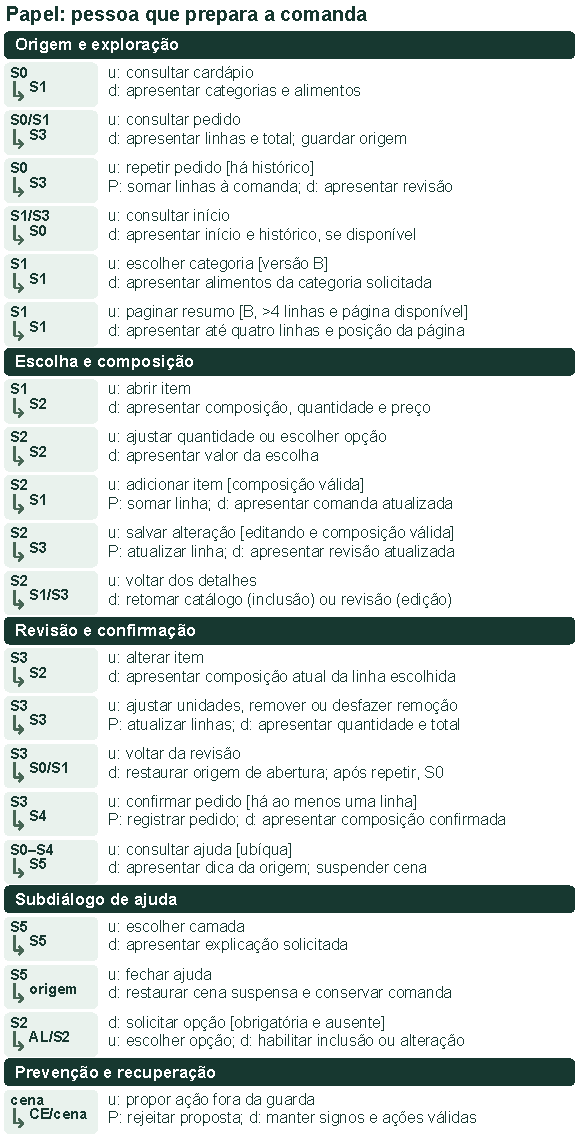
\includegraphics[width=\columnwidth]{../design/figures/MoLIC.pdf}
\par\smallskip\noindent\textbf{Esboços.} Cada quadro mostra a hierarquia dos signos e o ponto de acesso ao suporte. A linha de um pedido concreto inclui opção, quantidade e valor. O painel de pesquisa fica fora da projeção do agente.
\par\smallskip\noindent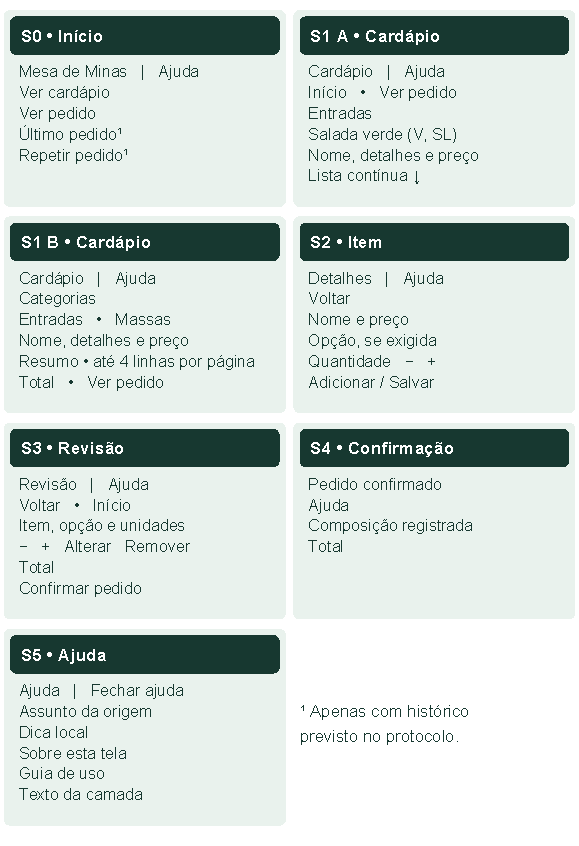
\includegraphics[width=\columnwidth]{../design/figures/Wireframes.pdf}
\section{Esquema conceitual de signos}
\noindent O esquema descreve cada signo usado nas tarefas pelo conteúdo e pela expressão. Não é o modelo de dados. A coluna \emph{Na observação do agente} aplica a equivalência de canal: \emph{trecho} é o texto geométrica e tipograficamente legível no recorte; abaixo do limiar de legibilidade restam o tipo do elemento e sua posição. Nenhum identificador interno, estado lógico de desabilitação ou elemento fora do recorte entra na observação. A coluna \emph{Evento} liga o signo ao registro do pesquisador. Os signos de aplicação recebem explicação completa nas três camadas da ajuda.
\newcommand{\SGhead}{\hline \textbf{Signo (entidade.atributo)} & \textbf{Origem} & \textbf{Conteúdo (tipo, restrições, default)} & \textbf{Expressão (widget)} & \textbf{Tipo} & \textbf{Na observação do agente} & \textbf{Evento}\\ \hline}
\begin{table*}[!t]
\caption{Esquema conceitual de signos estendido (parte 1: cardápio, item e navegação)}
\label{tab:signos1}
\centering\scriptsize\setlength{\tabcolsep}{3pt}\renewcommand{\arraystretch}{1.08}
\begin{tabularx}{\textwidth}{@{}>{\raggedright\arraybackslash}p{.135\textwidth}>{\raggedright\arraybackslash}p{.085\textwidth}>{\raggedright\arraybackslash}X>{\raggedright\arraybackslash}p{.15\textwidth}>{\raggedright\arraybackslash}p{.085\textwidth}>{\raggedright\arraybackslash}p{.165\textwidth}>{\raggedright\arraybackslash}p{.13\textwidth}@{}}
\SGhead
Restaurante.nome & domínio & texto; denominação do restaurante ou da lanchonete de treino & cabeçalho & estático & trecho legível & \UXev{elemento_visto}\\
Tela.assunto & aplicação & enumerado S0--S5; cena corrente & título da tela & estático & trecho do título & \UXev{tela_alterada}\\
Início.histórico & domínio & lista das linhas do último pedido, quando prevista na tarefa & relação de itens & estático & trechos de linhas & \UXev{elemento_visto}\\
Pedido.repetição & aplicação & ação; acrescenta as linhas históricas às atuais & botão Repetir pedido & estático & alvo visível & \UXev{item_adicionado}\\
Navegação.destino & convencional & enumerado: início, cardápio ou revisão & controles de navegação & estático & alvo visível & \UXev{tela_alterada}\\
Navegação.retorno & convencional & ação; abandona edição pendente & botão Voltar & estático & gesto ou alvo corrente & \UXev{tela_alterada}\\
Categoria.nome & domínio & texto; cinco categorias na ordem herdada & seção (A) ou aba (B) & estático & trecho & \UXev{elemento_visto}\\
Categoria.ativa & aplicação & enumerado; default: entradas (somente B) & realce da aba & dinâmico & pistas visíveis e itens expostos & \UXev{tela_alterada}\\
Item.nome & domínio & texto do catálogo; 30 itens & cabeçalho do cartão & estático & trecho, sem completar vizinhos & \UXev{elemento_visto}\\
Item.descrição & domínio & texto; ingredientes ou preparo & texto do cartão & estático & trecho & \UXev{elemento_visto}\\
Item.etiquetas & transformado & conjunto de \{V, SL, SA\}, possivelmente vazio & marcas junto ao item & metalinguístico & somente o próprio trecho & \UXev{elemento_visto}\\
Item.preço & domínio & centavos inteiros positivos; dois preços para massas & valor em reais & estático & trecho monetário & \UXev{elemento_visto}\\
Item.detalhes & aplicação & ação; abre a composição do item tocado & cartão tocável & estático & alvo visível, sem identificador interno & \UXev{tela_alterada}\\
Item.opção & domínio & tamanho ou acompanhamento obrigatório; default: nenhuma escolha & grupo de opções & dinâmico & textos expostos & \UXev{opcao_selecionada}\\
Opção.exigência & aplicação & condição para incluir o item & aviso escrito & metalinguístico & trecho do aviso, sem marca lógica de desabilitação & \UXev{elemento_visto}\\
Item.quantidade & domínio & inteiro $\geq 1$ & número e controles $+/-$ & dinâmico & número ou sinal visível & \UXev{acao_executada}\\
Item.inclusão & aplicação & ação; efetiva uma nova linha & botão Adicionar & dinâmico & alvo visível admissível & \UXev{item_adicionado}\\ \hline
\end{tabularx}
\end{table*}
\begin{table*}[!t]
\caption{Esquema conceitual de signos estendido (parte 2: pedido, ajuda, vista e protocolo)}
\label{tab:signos2}
\centering\scriptsize\setlength{\tabcolsep}{3pt}\renewcommand{\arraystretch}{1.08}
\begin{tabularx}{\textwidth}{@{}>{\raggedright\arraybackslash}p{.135\textwidth}>{\raggedright\arraybackslash}p{.085\textwidth}>{\raggedright\arraybackslash}X>{\raggedright\arraybackslash}p{.15\textwidth}>{\raggedright\arraybackslash}p{.085\textwidth}>{\raggedright\arraybackslash}p{.165\textwidth}>{\raggedright\arraybackslash}p{.13\textwidth}@{}}
\SGhead
Pedido.resumo & transformado & composição e total; somente em B & rodapé fixo & dinâmico & apenas a interseção efetiva com o recorte & \UXev{elemento_visto}\\
Resumo.página & aplicação & até quatro linhas por página; Anterior/Próxima quando há página nessa direção & paginação do rodapé (B) & dinâmico & alvos e linhas expostos & \UXev{acao_executada}\\
Linha.composição & transformado & nome, opção, unidades e subtotal & linha da revisão & dinâmico & fragmentos expostos & \UXev{elemento_visto}\\
Linha.unidades & transformado & inteiro positivo da linha existente & controles $+/-$ & dinâmico & controle visível & \UXev{item_alterado}\\
Linha.edição & aplicação & ação; reabre os detalhes da linha e aplica a mudança & botões Alterar e Salvar alteração & dinâmico & alvo do recorte & \UXev{item_alterado}\\
Linha.remoção & aplicação & ação; exclui a linha escolhida & botão Remover & dinâmico & alvo visível & \UXev{item_removido}\\
Linha.reposição & aplicação & ação; recupera a última remoção disponível & botão Desfazer remoção & dinâmico & alvo visível & \UXev{item_adicionado}\\
Pedido.total & transformado & soma dos subtotais, em reais & valor total & dinâmico & trecho & \UXev{elemento_visto}\\
Pedido.vazio & aplicação & ausência de linhas & mensagem & dinâmico & trecho & \UXev{elemento_visto}\\
Pedido.registro & aplicação & ação; exige comanda não vazia & botão Confirmar pedido, depois mensagem e linhas & dinâmico & alvo e resposta no recorte & \UXev{pedido_confirmado}\\
Ajuda.acesso & aplicação & ação; solicita explicação da cena & botão Ajuda ou F1 & estático & alvo visível ou acesso ubíquo previsto & \UXev{ajuda_aberta}\\
Ajuda.camada & aplicação & enumerado: dica local, sobre esta tela, guia de uso & três escolhas & dinâmico & opções da ajuda aberta & \UXev{ajuda_aberta}\\
Ajuda.tópico & aplicação & texto do assunto da cena de origem na camada escolhida & título e texto & metalinguístico & trecho, somente após a abertura & \UXev{observacao}\\
Ajuda.retorno & convencional & ação; retoma a cena de origem & botão Fechar ajuda ou Esc & estático & alvo visível & \UXev{ajuda_fechada}\\
Vista.escala e posição & convencional & janela de $360/z$ por $800/z$ px CSS e posição & gestos de ampliar, reduzir e deslocar & dinâmico & recorte e gestos permitidos & \UXev{zoom_alterado}, \UXev{vista_deslocada}\\
Protocolo.instrução & aplicação & enunciado literal e estável da tarefa & texto do protocolo & metalinguístico & texto literal & \UXev{tarefa_iniciada}\\
Protocolo.saída & convencional & ação; interromper por iniciativa própria & gesto Desistir & dinâmico & gesto de protocolo & \UXev{desistencia}\\ \hline
\end{tabularx}
\end{table*}

\section{Texto das três camadas de ajuda}
\par\smallskip\noindent\textbf{S0}
\par\noindent\emph{Dica local.} Consulte o cardápio para começar. Se houver um último pedido, você pode consultá-lo aqui.
\par\noindent\emph{Sobre esta tela.} O último pedido mostra a composição registrada anteriormente. Repetir pedido acrescenta esses itens ao pedido em andamento. Confira também os itens que já estavam nele.
\par\noindent\emph{Guia de uso.} Para começar de novo pelo cardápio, escolha Ver cardápio. Para usar uma composição anterior, escolha Repetir pedido, se disponível. Na revisão, confira as opções e as quantidades. O pedido é registrado quando você o confirma.
\par\smallskip\noindent\textbf{S1}
\par\noindent\emph{Dica local.} Cada item tem nome, descrição e preço. Consulte o item para conhecer as opções disponíveis.
\par\noindent\emph{Sobre esta tela.} Na lista contínua, os itens aparecem por categoria. Na versão com categorias, escolha o nome da categoria para ver seus itens. Ver pedido abre a revisão. O resumo no rodapé, quando presente, acompanha o pedido em andamento.
\par\noindent\emph{Guia de uso.} As etiquetas pertencem ao item junto do qual aparecem. (V) significa vegetariano, (SL) significa sem lactose e (SA) significa sem açúcar ou sem açúcar adicionado. Consulte os detalhes, escolha as opções desejadas e acrescente o item. Você pode rever o pedido antes de confirmar.
\par\smallskip\noindent\textbf{S2}
\par\noindent\emph{Dica local.} Confira o nome e o preço do item. Quando houver uma opção obrigatória, escolha-a antes de acrescentar ou salvar.
\par\noindent\emph{Sobre esta tela.} O acompanhamento compõe o prato principal. O tamanho define a porção de massa. A quantidade indica quantas unidades da combinação serão pedidas. Aumente ou diminua a quantidade pelos controles junto ao número.
\par\noindent\emph{Guia de uso.} Ao incluir um item, escolha a opção, ajuste a quantidade e use Adicionar. Ao modificar uma linha existente, use Salvar alteração. Para sair dos detalhes antes de aplicar a escolha, use Voltar.
\par\smallskip\noindent\textbf{S3}
\par\noindent\emph{Dica local.} Confira cada linha, suas opções e quantidades. O total reúne todas as linhas do pedido.
\par\noindent\emph{Sobre esta tela.} Use os controles junto à quantidade para ajustá-la. Alterar permite rever as opções da linha. Remover retira a linha do pedido. Confira o nome junto dos controles antes de fazer uma alteração.
\par\noindent\emph{Guia de uso.} Percorra o pedido e confira as linhas com o que deseja receber. Para recuperar uma linha, use Desfazer remoção enquanto essa opção estiver disponível. Você também pode voltar ao cardápio e acrescentar o item novamente. Ao terminar a conferência, use Confirmar pedido.
\par\smallskip\noindent\textbf{S4}
\par\noindent\emph{Dica local.} A confirmação indica que o pedido foi registrado.
\par\noindent\emph{Sobre esta tela.} O registro conclui a composição do pedido neste restaurante fictício. A confirmação informa que a operação terminou.
\par\noindent\emph{Guia de uso.} Consulte a mensagem de confirmação para reconhecer o fim do pedido. Esta demonstração não processa pagamentos nem envia pedidos a restaurantes.

\section{Rastreabilidade e registro de decisões}
\begin{uxtable}{Perfil e tarefa}{Mecanismo, signo, registro e estatuto}
\UXrow{M1, C1\,1 e 4}{Ampliação $\rightarrow$ recorte e legibilidade $\rightarrow$ nome/preço $\rightarrow$ deslocamentos por item ($D$). E para amplitude observada, HO para limiar e geometria.}
\UXrow{M2, C1\,2}{Contexto ausente $\rightarrow$ memória FIFO de fragmentos $\rightarrow$ comparação de preços $\rightarrow$ revisita ($V$). E indireta para perda do contexto, HO para $k$.}
\UXrow{M3, C1\,1.2}{Nome fora da vista $\rightarrow$ atributo sem herdar rótulo $\rightarrow$ item vizinho $\rightarrow Re_{E2}$. HO para a associação operacional.}
\UXrow{M4, deslocar}{Gestos não intencionais $\rightarrow$ toque no início do deslocamento $\rightarrow$ abertura e retorno $\rightarrow Re_{E4},A$. E para o fenômeno, HO para $p=0{,}05$.}
\UXrow{M5, C2\,2}{Linha de revisão fora da vista $\rightarrow$ somente trechos vistos e memória $\rightarrow$ divergência final $\rightarrow Re_{E5}$. HO para posição e efeito.}
\UXrow{M6, C1\,1.2}{Varredura $\rightarrow$ restrição de deslocamentos $\rightarrow$ sequência de itens expostos $\rightarrow O,D$. E para estratégias em outra tarefa, HO para transferência.}
\UXrow{M7, impasse}{Busca de suporte $\rightarrow$ estagnação e acionamento $\rightarrow$ ajuda por camada $\rightarrow U$. HO para $n,q$ e igualdade P/C.}
\end{uxtable}
\begin{uxtable}{Questão e opções}{Critério, decisão e estatuto}
\UXrow{Conferência separada ou persistente?}{Consultar a comanda durante a escolha. Preservar as duas versões herdadas. Composição persistente pode poupar navegação ou cobrir alimentos. HO; aferir no estudo futuro.}
\UXrow{Bloquear ou avisar?}{Opção obrigatória define uma composição válida. Usar PP, PA e RA para essa operação. Para etiquetas e orçamento, manter edição sem bloqueio específico. PD; comparar somente oportunidades equivalentes.}
\UXrow{Associação implícita ou nome sugerido?}{Se o nome não cabe no recorte, a observação conserva somente a parte visível. PD para paridade, HO para truncamento.}
\UXrow{Ajuda espontânea ou solicitada?}{Preservar iniciativa e medir suporte. Texto comum em três camadas, acessado por ação registrada. PD. O acionador da política tem parâmetros independentes, HO.}
\UXrow{Contar exposição ou inferir leitura?}{A caixa pode interceptar a vista antes de um termo inteiro ser legível. Registrar fração e distinguir exposição de decisão interna. HO.}
\UXrow{Último pedido substitui ou soma?}{V2 exige identificar residual já presente. Repetir conserva as linhas existentes; oferecer conferência e recuperação. PD diretamente herdado da operação congelada.}
\UXrow{Concluir por fala ou composição?}{Registrar confirmação; o verificador examina o estado final segundo as regras herdadas. PD. Uma correção anterior não apaga o erro registrado.}
\end{uxtable}


\end{document}
